\documentclass[12pt, xcolor=dvipsnames,svgnames,x11names]{article}

\usepackage{tikz}
\usepackage{pgfplots}
\usepackage{minted}





\def\m@th{\normalcolor\mathsurround\z@}

\setlength{\parskip}{\baselineskip}%
\setlength{\parindent}{0pt}%

\def\e{{\textrm{e}}}
\def\d{\textrm{d}}
\def\T{{\textsf{T}}}
\def\sech{{\textrm{sech}}}
\def\x{{\mathbf x}}

\def\++{{$^{++}$}}

\def\Abb{{\mathbb A}}
\def\Bbb{{\mathbb B}}
\def\Cbb{{\mathbb C}}
\def\Dbb{{\mathbb D}}
\def\Ebb{{\mathbb E}}
\def\Fbb{{\mathbb F}}
\def\Gbb{{\mathbb G}}
\def\Hbb{{\mathbb H}}
\def\Ibb{{\mathbb I}}
\def\Jbb{{\mathbb J}}
\def\Kbb{{\mathbb K}}
\def\Lbb{{\mathbb L}}
\def\Mbb{{\mathbb M}}
\def\Nbb{{\mathbb N}}
\def\Obb{{\mathbb O}}
\def\Pbb{{\mathbb P}}
\def\Qbb{{\mathbb Q}}
\def\Rbb{{\mathbb R}}
\def\Sbb{{\mathbb S}}
\def\Tbb{{\mathbb T}}
\def\Ubb{{\mathbb U}}
\def\Vbb{{\mathbb V}}
\def\Wbb{{\mathbb W}}
\def\Xbb{{\mathbb X}}
\def\Ybb{{\mathbb Y}}
\def\Zbb{{\mathbb Z}}



\def\Acal{{\mathcal A}}
\def\Bcal{{\mathcal B}}
\def\Ccal{{\mathcal C}}
\def\Dcal{{\mathcal D}}
\def\Ecal{{\mathcal E}}
\def\Fcal{{\mathcal F}}
\def\Gcal{{\mathcal G}}
\def\Hcal{{\mathcal H}}
\def\Ical{{\mathcal I}}
\def\Jcal{{\mathcal J}}
\def\Kcal{{\mathcal K}}
\def\Lcal{{\mathcal L}}
\def\Mcal{{\mathcal M}}
\def\Ncal{{\mathcal N}}
\def\Ocal{{\mathcal O}}
\def\Pcal{{\mathcal P}}
\def\Qcal{{\mathcal Q}}
\def\Rcal{{\mathcal R}}
\def\Scal{{\mathcal S}}
\def\Tcal{{\mathcal T}}
\def\Ucal{{\mathcal U}}
\def\Vcal{{\mathcal V}}
\def\Wcal{{\mathcal W}}
\def\Xcal{{\mathcal X}}
\def\Ycal{{\mathcal Y}}
\def\Zcal{{\mathcal Z}}

\def\abf{{\mathbf a}}
\def\bbf{{\mathbf b}}
\def\cbf{{\mathbf c}}
\def\dbf{{\mathbf d}}
\def\ebf{{\mathbf e}}
\def\fbf{{\mathbf f}}
\def\gbf{{\mathbf g}}
\def\hbf{{\mathbf h}}
\def\ibf{{\mathbf i}}
\def\jbf{{\mathbf j}}
\def\kbf{{\mathbf k}}
\def\lbf{{\mathbf l}}
\def\mbf{{\mathbf m}}
\def\nbf{{\mathbf n}}
\def\obf{{\mathbf o}}
\def\pbf{{\mathbf p}}
\def\qbf{{\mathbf q}}
\def\rbf{{\mathbf r}}
\def\sbf{{\mathbf s}}
\def\tbf{{\mathbf t}}
\def\ubf{{\mathbf u}}
\def\vbf{{\mathbf v}}
\def\wbf{{\mathbf w}}
\def\xbf{{\mathbf x}}
\def\ybf{{\mathbf y}}
\def\zbf{{\mathbf z}}

\def\Abf{{\mathbf A}}
\def\Bbf{{\mathbf B}}
\def\Cbf{{\mathbf C}}
\def\Dbf{{\mathbf D}}
\def\Ebf{{\mathbf E}}
\def\Fbf{{\mathbf F}}
\def\Gbf{{\mathbf G}}
\def\Hbf{{\mathbf H}}
\def\Ibf{{\mathbf I}}
\def\Jbf{{\mathbf J}}
\def\Kbf{{\mathbf K}}
\def\Lbf{{\mathbf L}}
\def\Mbf{{\mathbf M}}
\def\Nbf{{\mathbf N}}
\def\Obf{{\mathbf O}}
\def\Pbf{{\mathbf P}}
\def\Qbf{{\mathbf Q}}
\def\Rbf{{\mathbf R}}
\def\Sbf{{\mathbf S}}
\def\Tbf{{\mathbf T}}
\def\Ubf{{\mathbf U}}
\def\Vbf{{\mathbf V}}
\def\Wbf{{\mathbf W}}
\def\Xbf{{\mathbf X}}
\def\Ybf{{\mathbf Y}}
\def\Zbf{{\mathbf Z}}

\def\phat{{\hat p}}

\usepackage{amsmath}
\DeclareMathOperator*{\argmax}{arg\,max}
\DeclareMathOperator*{\argmin}{arg\,min}

\def\xbar{{\overline x}}
\def\ybar{{\overline y}}
\def\e{{\textrm{e}}}
\def\d{\textrm{d}}
\def\T{{\textsf{T}}}
\def\sech{{\textrm{sech}}}
\def\x{{\mathbf x}}

\def\++{{$^{++}$}}

\def\Abb{{\mathbb A}}
\def\Bbb{{\mathbb B}}
\def\Cbb{{\mathbb C}}
\def\Dbb{{\mathbb D}}
\def\Ebb{{\mathbb E}}
\def\Fbb{{\mathbb F}}
\def\Gbb{{\mathbb G}}
\def\Hbb{{\mathbb H}}
\def\Ibb{{\mathbb I}}
\def\Jbb{{\mathbb J}}
\def\Kbb{{\mathbb K}}
\def\Lbb{{\mathbb L}}
\def\Mbb{{\mathbb M}}
\def\Nbb{{\mathbb N}}
\def\Obb{{\mathbb O}}
\def\Pbb{{\mathbb P}}
\def\Qbb{{\mathbb Q}}
\def\Rbb{{\mathbb R}}
\def\Sbb{{\mathbb S}}
\def\Tbb{{\mathbb T}}
\def\Ubb{{\mathbb U}}
\def\Vbb{{\mathbb V}}
\def\Wbb{{\mathbb W}}
\def\Xbb{{\mathbb X}}
\def\Ybb{{\mathbb Y}}
\def\Zbb{{\mathbb Z}}



\def\Acal{{\mathcal A}}
\def\Bcal{{\mathcal B}}
\def\Ccal{{\mathcal C}}
\def\Dcal{{\mathcal D}}
\def\Ecal{{\mathcal E}}
\def\Fcal{{\mathcal F}}
\def\Gcal{{\mathcal G}}
\def\Hcal{{\mathcal H}}
\def\Ical{{\mathcal I}}
\def\Jcal{{\mathcal J}}
\def\Kcal{{\mathcal K}}
\def\Lcal{{\mathcal L}}
\def\Mcal{{\mathcal M}}
\def\Ncal{{\mathcal N}}
\def\Ocal{{\mathcal O}}
\def\Pcal{{\mathcal P}}
\def\Qcal{{\mathcal Q}}
\def\Rcal{{\mathcal R}}
\def\Scal{{\mathcal S}}
\def\Tcal{{\mathcal T}}
\def\Ucal{{\mathcal U}}
\def\Vcal{{\mathcal V}}
\def\Wcal{{\mathcal W}}
\def\Xcal{{\mathcal X}}
\def\Ycal{{\mathcal Y}}
\def\Zcal{{\mathcal Z}}

\def\abf{{\mathbf a}}
\def\bbf{{\mathbf b}}
\def\cbf{{\mathbf c}}
\def\dbf{{\mathbf d}}
\def\ebf{{\mathbf e}}
\def\fbf{{\mathbf f}}
\def\gbf{{\mathbf g}}
\def\hbf{{\mathbf h}}
\def\ibf{{\mathbf i}}
\def\jbf{{\mathbf j}}
\def\kbf{{\mathbf k}}
\def\lbf{{\mathbf l}}
\def\mbf{{\mathbf m}}
\def\nbf{{\mathbf n}}
\def\obf{{\mathbf o}}
\def\pbf{{\mathbf p}}
\def\qbf{{\mathbf q}}
\def\rbf{{\mathbf r}}
\def\sbf{{\mathbf s}}
\def\tbf{{\mathbf t}}
\def\ubf{{\mathbf u}}
\def\vbf{{\mathbf v}}
\def\wbf{{\mathbf w}}
\def\xbf{{\mathbf x}}
\def\ybf{{\mathbf y}}
\def\zbf{{\mathbf z}}

\def\Abf{{\mathbf A}}
\def\Bbf{{\mathbf B}}
\def\Cbf{{\mathbf C}}
\def\Dbf{{\mathbf D}}
\def\Ebf{{\mathbf E}}
\def\Fbf{{\mathbf F}}
\def\Gbf{{\mathbf G}}
\def\Hbf{{\mathbf H}}
\def\Ibf{{\mathbf I}}
\def\Jbf{{\mathbf J}}
\def\Kbf{{\mathbf K}}
\def\Lbf{{\mathbf L}}
\def\Mbf{{\mathbf M}}
\def\Nbf{{\mathbf N}}
\def\Obf{{\mathbf O}}
\def\Pbf{{\mathbf P}}
\def\Qbf{{\mathbf Q}}
\def\Rbf{{\mathbf R}}
\def\Sbf{{\mathbf S}}
\def\Tbf{{\mathbf T}}
\def\Ubf{{\mathbf U}}
\def\Vbf{{\mathbf V}}
\def\Wbf{{\mathbf W}}
\def\Xbf{{\mathbf X}}
\def\Ybf{{\mathbf Y}}
\def\Zbf{{\mathbf Z}}

\def\phat{{\hat p}}
\def\what{{\hat w}}
\def\yhat{{\hat y}}


\newcommand{\answer}{
    \fcolorbox{orange}{PapayaWhip}{
\begin{minipage}{\textwidth}
        \textbf{Answer}
    \end{minipage}
}
}

\newcommand{\codeoutput}[1]{
Output:\\\vspace{5px}
    \fcolorbox{orange}{WhiteSmoke}{
\begin{minipage}{\textwidth}
        { \color{DodgerBlue} 
        
        
       \texttt{#1}
       }
    \end{minipage}
}
}


\newcommand{\orangebox}[1]{
    \fcolorbox{orange}{white}{
\begin{minipage}{\textwidth}
       {\color{MidnightBlue} 
       #1
       }
    \end{minipage}
}
}


\definecolor{lightapricot}{rgb}{0.99, 0.84, 0.69}
\definecolor{lightblue}{rgb}{0.68, 0.85, 0.90}
\definecolor{blanchedalmond}{rgb}{1.0, 0.92, 0.8}
\definecolor{blizzardblue}{rgb}{0.67, 0.9, 0.93}
\definecolor{blond}{rgb}{0.98, 0.94, 0.75}
\definecolor{babyblueeyes}{rgb}{0.63, 0.79, 0.95}
\definecolor{babypink}{rgb}{0.96, 0.76, 0.76}
\definecolor{bananamania}{rgb}{0.98, 0.91, 0.71}
\definecolor{beaublue}{rgb}{0.74, 0.83, 0.9}
\definecolor{antiquewhite}{rgb}{0.98, 0.92, 0.84}
\definecolor{anti-flashwhite}{rgb}{0.95, 0.95, 0.96}
\definecolor{brightlavender}{rgb}{0.75, 0.58, 0.89}
\definecolor{brightube}{rgb}{0.82, 0.62, 0.91}
\definecolor{brilliantlavender}{rgb}{0.96, 0.73, 1.0}
\definecolor{lightcerulean}{rgb}{0.11, 0.67, 0.84}
\definecolor{cpeyellow}{HTML}{F5F5DC}                 % Beige (much softer)
\definecolor{powderGreen}{HTML}{F0F8E8}               % Very pale mint


% Darker versions of the original colors
\definecolor{deepapricot}{rgb}{0.85, 0.65, 0.45}        % darker lightapricot
\definecolor{deepblue}{rgb}{0.45, 0.65, 0.75}           % darker lightblue
\definecolor{toastedalmond}{rgb}{0.85, 0.75, 0.60}      % darker blanchedalmond
\definecolor{stormblue}{rgb}{0.45, 0.70, 0.75}          % darker blizzardblue
\definecolor{goldenrod}{rgb}{0.80, 0.75, 0.50}          % darker blond
\definecolor{royalblue}{rgb}{0.40, 0.60, 0.80}          % darker babyblueeyes
\definecolor{rosewood}{rgb}{0.75, 0.45, 0.45}           % darker babypink
\definecolor{mustardyellow}{rgb}{0.80, 0.70, 0.45}      % darker bananamania
\definecolor{navyblue}{rgb}{0.50, 0.60, 0.70}           % darker beaublue
\definecolor{antiquetan}{rgb}{0.80, 0.70, 0.60}         % darker antiquewhite
\definecolor{silvergray}{rgb}{0.75, 0.75, 0.80}         % darker anti-flashwhite
\definecolor{darklavender}{rgb}{0.55, 0.35, 0.70}       % darker brightlavender
\definecolor{deepube}{rgb}{0.65, 0.40, 0.75}            % darker brightube
\definecolor{plumviolet}{rgb}{0.75, 0.50, 0.85}         % darker brilliantlavender
\definecolor{deepcerulean}{rgb}{0.08, 0.45, 0.65}       % darker lightcerulean

\definecolor{roseRed}{HTML}{e20047}
\definecolor{coolGray}{HTML}{474747} % Neutral gray to contrast roseRed
\definecolor{mocha}{HTML}{a47864}
\definecolor{sage}{HTML}{8a9a5b}
\definecolor{dustyblue}{HTML}{6e8ca0}
\definecolor{terracotta}{HTML}{c87f5b}
\definecolor{lavender}{HTML}{9d8bb0}
\definecolor{darkmocha}{HTML}{7a5a4b}
\definecolor{darksage}{HTML}{667244}
\definecolor{darkdustyblue}{HTML}{526878}
\definecolor{darkterracotta}{HTML}{9e6347}
\definecolor{darklavender}{HTML}{766688}
\definecolor{winery}{HTML}{7e212a}

% ---- Title header palette ----
\definecolor{hdrplum}{HTML}{2E0014}    % near-black plum, header band
\definecolor{hdrcoral}{HTML}{E17564}   % coral, accent rules
\definecolor{hdrslate}{HTML}{2F4F4F}   % dark slate grey, frame and body text
\colorlet{hdrslatetint}{hdrslate!12!white}
\colorlet{hdrcoraltint}{hdrcoral!15!white}

\usepackage{sectsty}
\sectionfont{\color{darklavender}}  % sets colour of sections
\subsectionfont{\color{plumviolet}}  % sets colour of sections
\subsubsectionfont{\color{deepube}}  % sets colour of sections

\usepackage{xcolor}
%\usepackage{universityos}
\usepackage{xspace}
\usepackage{url}
\usepackage[colorlinks=true,bookmarks=false,linkcolor=black,urlcolor=blue,citecolor=black]{hyperref}
\usepackage{fancyhdr}
\usepackage[top=1in,bottom=1in,left=1in,right=1in]{geometry}
\usepackage{multicol}
\usepackage{pgfplots}
\usetikzlibrary{circuits.logic.US}
% ---- Typography: Palatino for text and math ----
% The previous version loaded mathpazo and then restored the old \rmdefault,
% so Palatino applied to math only. The lines below apply it to the text too.
\usepackage[T1]{fontenc}
\usepackage[sc]{mathpazo}   % Palatino text + math, with real small caps
\linespread{1.05}           % Palatino has a large x-height, so open up the leading
\usepackage[scaled=0.92]{helvet}  % companion sans, used by \textsf
\renewcommand{\ttdefault}{cmtt}    % keep Computer Modern Typewriter for code

\usepackage{eso-pic}



\usetikzlibrary{calc}
\usepackage{circuitikz}



\usepackage[many]{tcolorbox}
\setlength{\parindent}{0pt}
\setlength{\parskip}{4pt}%

\newcommand{\coursenumber}{CPE 486/586}
\newcommand{\courseyear}{2026\xspace}
\newcommand{\coursedatetime}{Tue/Thur 11:20 AM -- 12:40 PM\xspace}
\newcommand{\coursetitle}{Machine Learning for Engineering Applications\xspace}
\newcommand{\courseterm}{Fall, \courseyear}
\newcommand{\instructorname}{Rahul Bhadani\xspace}
\newcommand{\instructoremail}{\href{mailto:rahul.bhadani@uah.edu}{rahul.bhadani@uah.edu}}
\newcommand{\instructoroffice}{ENG 217-H\xspace}


\newtcolorbox{answerbox}{
  enhanced,
  breakable,
  sharp corners=northwest,
  sharp corners=southeast,
  colback=white,
  colframe=red!75!black,
  halign=left, 
  boxrule=2pt, 
  left=1em, 
  right=1em, 
  top=0.5em, 
  bottom=0.5em, 
  drop shadow=coolGray,
  title=Answer
}

\renewcommand{\familydefault}{\rmdefault}   % Palatino (loaded in common.tex)


% Redefine \maketitle to include tcolorbox
% Palette: hdrplum (2E0014), hdrcoral (E17564), hdrslate (2F4F4F)
\makeatletter
\newcommand{\hdrrule}{{\color{hdrcoral}\rule{4.5em}{1.1pt}}}
\renewcommand{\maketitle}{%
      \begin{center}
         \begin{tcolorbox}[
               enhanced,
               colback=white,
               colframe=hdrslate,
               boxrule=0.8pt,
               arc=4pt,
               left=0pt,
               right=0pt,
               top=0pt,
               bottom=0pt,
               drop shadow={hdrslate!35!white},
         ]
               % Header band: deep plum with a coral baseline
               \begin{tcolorbox}[
                  enhanced,
                  colback=hdrplum,
                  colframe=hdrplum,
                  boxrule=0pt,
                  arc=4pt,
                  sharp corners=south,
                  left=2em,
                  right=2em,
                  top=1.1em,
                  bottom=1.1em,
                  borderline south={2.2pt}{0pt}{hdrcoral},
               ]
                  \centering
                  % Palatino has no bold small caps, so the title stays at medium
                  % weight and gains presence from size and the dark band instead.
                  {\LARGE\color{white}\linespread{1.25}\selectfont\@title}
               \end{tcolorbox}

               % Body: author, coral divider, then the due information
               \vspace{1.1em}
               \centering
               {\large\color{hdrslate}\@author}\\[0.7em]
               \hdrrule\\[0.7em]
               {\normalsize\color{hdrplum}\@date}
               \vspace{1.1em}
         \end{tcolorbox}
      \end{center}
      \vspace{1.5em}
}
\makeatother




\newcommand{\hw}{Homework 5:\\\normalsize SVM, PCA, Classification, and Neural Network}
\newcommand{\duedate}{November 26, 2026, 11:59 PM}

\newenvironment{multiequation}[1][]{%
\begin{equation}%
   \begin{aligned}%
   \ifx#1\@empty\else\label{#1}\fi%
}{%
   \end{aligned}%
\end{equation}%
}
\pagestyle{fancy}

\lhead{\footnotesize{\coursenumber, \courseterm}, \footnotesize{UAH}}
\chead{}
\rhead{\footnotesize{\emph{\hw}}}
\lfoot{\footnotesize{\instructorname}}
\cfoot{\footnotesize{\thepage}}
\rfoot{\footnotesize{\textit{Last Revised:~\today}}}
\renewcommand{\headrulewidth}{0.1pt}
\renewcommand{\footrulewidth}{0.1pt}
\newcommand{\minipagewidth}{0.8\columnwidth}

\renewcommand{\thefootnote}{\fnsymbol{footnote}}


\renewcommand{\headrulewidth}{0.1pt}
\renewcommand{\footrulewidth}{0.1pt}

\renewcommand{\thefootnote}{\fnsymbol{footnote}}




\begin{document}


\title{\textsc{\hw\\
\coursenumber}}
\author{Instructor: \instructorname}
\date{Due: \duedate\\ 135oints}

\maketitle

\setlength{\unitlength}{1in}
You are allowed to use a generative model-based AI tool for your assignment. However, you must submit an accompanying reflection report detailing how you used the AI tool, the specific query you made, and how it improved your understanding of the subject. You are also required to submit screenshots of your conversation with any large language model (LLM) or equivalent conversational AI, clearly showing the prompts and your login avatar. Some conversational AIs provide a way to share a conversation link, and such a link is desirable for authenticity. Failure to do so may result in actions taken in compliance with the plagiarism policy.

Additionally, you must include your thoughts on how you would approach the assignment if such a tool were not available. Failure to provide a reflection report for every assignment where an AI tool is used may result in a penalty, and subsequent actions will be taken in line with the plagiarism policy.

\subsection*{Submission instruction:}
You may either complete your entire homework on Python Notebook  and submit a Google Colab link or you may choose a combination of a pdf and Google Colab Notebook. However, you must provide \textbf{publicly accessible} Google Colab URL on Canvas.

For .pdf on Canvas, follow the format  \texttt{CPE486586-LastFirst-HW-XX}. For example, if your name is Sam Wells, your file name should be \texttt{CPE486586-WellsSam-HW-XX.pdf}.

Your submission must contain your name and UAH Charger ID or your UAH email address.  Please number your pages as well.

\textbf{Please write down your unique keyword corresponding to your package and your Github account URL. Do not provide a link to your Google Colab notebook. Upload your Google colab notebook to your repo in a new folder called \textbf{HWNotebooks}. Provide your GitHub commit hash. Your submitted notebook must be fully executed with all cells outputs. Please make sure there are no error in your submitted notebook.}

\vskip 1em
\hrule
\vskip 1em


% {\LARGE \color{stormblue} \textbf{Python Practice-I}}


{{\LARGE \textbf{Theory}}}


\section{Distance between Hyperplanes (5 points)}
Consider two hyperplanes:

$$
H_1: \wbf^\top \xbf = 52
$$
and

$$
H_2: \wbf^\top \xbf = 64
$$

where $w$ is unknown.

What is the distance between the two hyperplanes $H_1$ and $H_2$?


\section{Overfitting in SVM (5 points)}
What strategy (such as a change in SVM formulation) would you take to avoid overfitting in the case of a Support Vector Machine?


\section{K-means (5 Points)}
Given $\{(1,2), (2,1), (4,5), (5,4) \}$, perform one iteration of K-mens with initial centroids at $(1,1)$ and $(5,5)$.


\section{Anomaly Detection in Clustering (5 Points)}
How would you use clustering techniques to detect anomaly?

\section{Single Neuron Forward Pass (10 Points)}
Calculate the output of a single neuron with:
\begin{itemize}
    \item Inputs: $x_1 = 0.5$, $x_2 = 0.8$, $x_3 = 0.2$
    \item Weights: $w_1 = 0.6$, $w_2 = -0.3$, $w_3 = 0.4$
    \item Bias: $b = 0.1$
    \item Activation: ReLU function $f(z) = \max(0, z)$
\end{itemize}
Calculate: $a = f\left(\sum_{i=1}^3 w_i x_i + b\right)$


\section{Neural Network by Hand (20 points)}
\label{sec:neuralnetbyhand}
Let's consider features of two training samples $\xbf = [\xbf^{(1)}, \xbf^{(2)}] = [(x_1^{(1)}, x_2^{(1)}), (x_1^{(2)}, x_2^{(2)})] = [ (2, 4), (4, 5)]$ and the response variable as $\ybf = [ y^{(1)}, y^{(2)}] = [-1, 1]$. Note that when we don't write superscript, i.e. $x_1$ or $x_2$, we are simply considering features of \textit{a} training sample without specifying which training sample.

Consider a classification problem for which we will develop a neural network model. The loss function to be considered is 

$$
\Lcal ( \ybf, \hat{\ybf}) = \Lcal = -\cfrac{1}{n} \sum_{i=1}^n \bigg ( y^{(i)} \log(\yhat^{(i)}) + (1- y^{(i)} )\log(1 - \yhat^{(i)} )  \bigg)
$$

Note that this is similar to the problem demonstrated in the class except we will calculate the loss by taking both training samples.

Here, 

$$
\cfrac{\partial \Lcal }{\yhat^{(1)}} = -\cfrac{y^{(1)}}{\yhat^{(1)}}  + \cfrac{1 - y^{(1)}}{1 - \yhat^{(1)}}
$$

and
$$
\cfrac{\partial \Lcal }{\yhat^{(2)}} = -\cfrac{y^{(2)}}{\yhat^{(2)}}  + \cfrac{1 - y^{(2)}}{1 - \yhat^{(2)}}
$$

Individual training sample $i$ will lead to the gradient with respect to a weight $W$ as:

\begin{equation}
\label{eq:gradient_per_sample}
    \begin{aligned}
\nabla_W \Lcal^{(i)} = \cfrac{\partial \Lcal }{W^{(i)}} = \cfrac{\partial \Lcal }{\yhat^{(i)}} \times \cfrac{\yhat^{(i)}} {\partial z^{(i)}} \times \cfrac{\partial z^{(i)}}{\partial W^{(i)} } 
    \end{aligned}
\end{equation}
In Equation~\eqref{eq:gradient_per_sample}, superscript $(i)$ denotes that gradient is calculated for individual samples. Then we calculate the average gradient as

\begin{equation}
    \begin{aligned}
        \nabla_W \Lcal = \cfrac{1}{n}\sum_i^n  \cfrac{\partial \Lcal }{W^{(i)}} 
    \end{aligned}
\end{equation}

so that the update rule for stochastic gradient descent becomes:
\begin{equation}
    \begin{aligned}
        W = W - \eta \nabla_W \Lcal
    \end{aligned}
\end{equation}

{\textcolor{red}{What it means is that you need to calculate the gradient for both training samples, take the average, and then update the weights.}}

                                                    
     Now, consider a neural network with one hidden layer containing three neurons so that the architecture looks as shown in Figure~\ref{fig:neuralnet}. In this problem, we won't consider bias, that is bias $b = 0$ at all neurons of the given Neural Network.

\label{eq:axis_max}
\begin{figure}
    \centering
   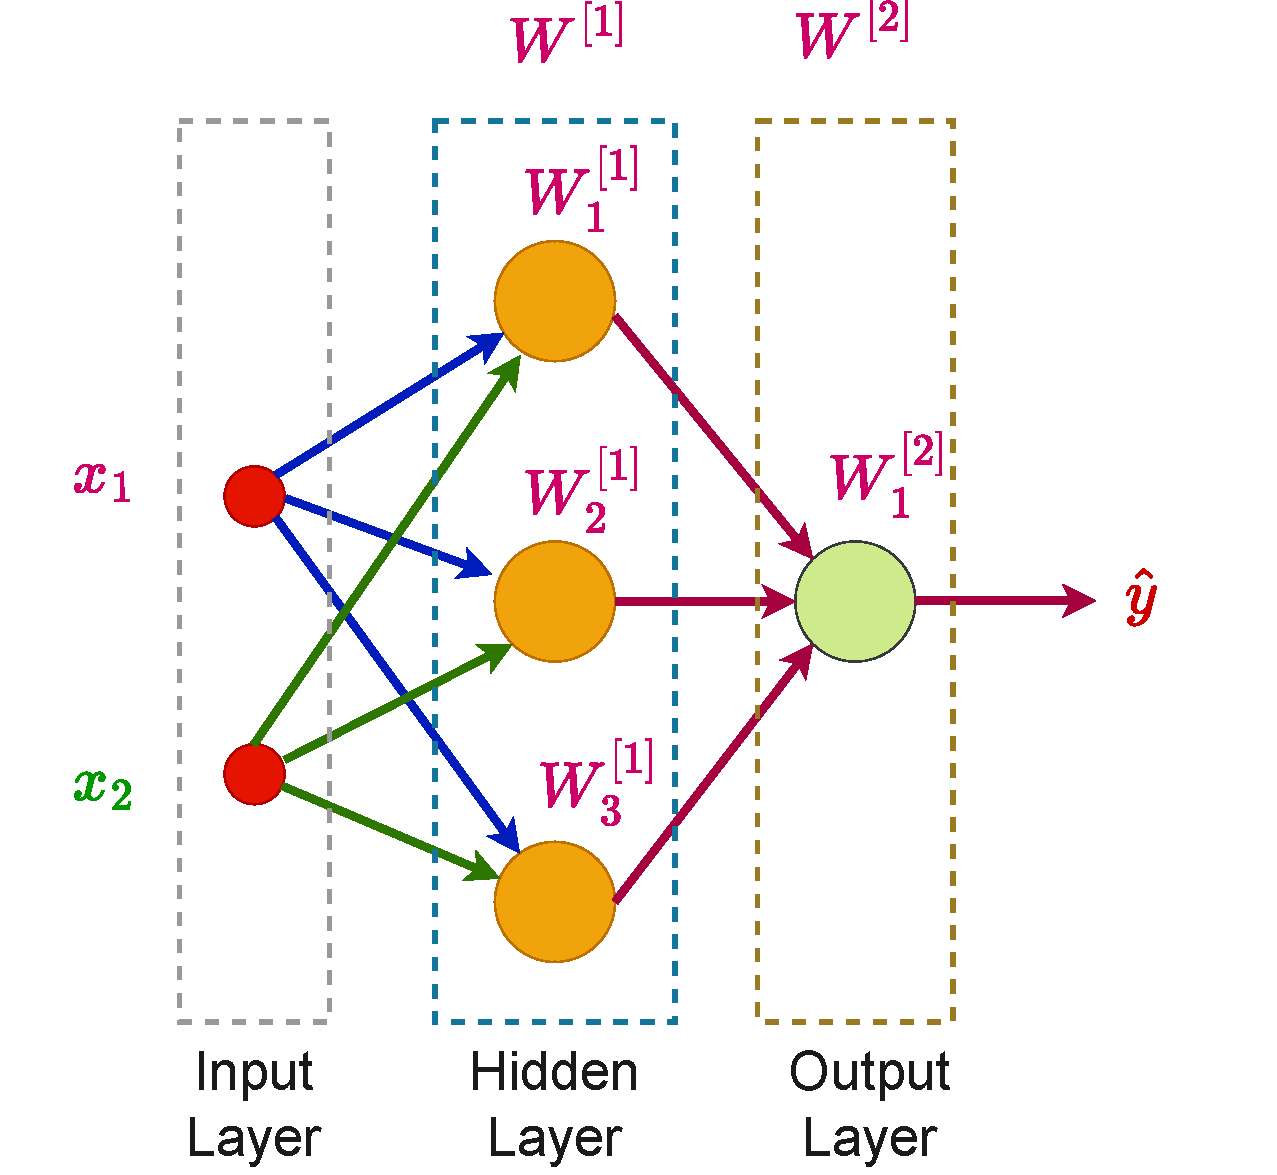
\includegraphics[width=0.60\textwidth]{../Lectures/figures/NeuralNet.pdf}
    \caption{\hw: Q\ref{sec:neuralnetbyhand}}
    \label{fig:neuralnet}
\end{figure}

Further, let's consider the following initial values of weights:

\begin{equation}
    \begin{aligned}
    W^{[1]}_1 & = [0.1, 0.3]\\
    W^{[1]}_2 & = [0.2, 0.4]\\
    W^{[1]}_3 & = [0.1, 0.5]\\
    W^{[2]}_1 & = [0.1, 0.2, 0.1]
    \end{aligned}
\end{equation}


Further, we will also consider the activation functions at all four neurons to be sigmoid, i.e.

$$
a = \sigma(z) = \cfrac{1}{1 + e^{-z}}
$$
Note that the derivative of $a$ with respect to $z$ is given 

$$
\cfrac{\partial a}{\partial z} = \sigma(z) \bigg( 1 - \sigma(z) \bigg) 
$$

You are required to complete the following task (only for one epoch) \textbf{(5 points each)}:

Use $\eta = 0.05$.

\begin{enumerate}
    \item Perform the forward propagation on the first hidden layer and write down $z_1^{[1]}$, $z_2^{[1]}$, $z_3^{[1]}$, $a_1^{[1]}$, $a_2^{[1]}$, and $a_3^{[1]}$ for \textbf{both training samples}.
    \item Perform the forward propagation on the output layer and write down $z_1^{[2]}$, $a_1^{[2]}$ for \textbf{both training samples}.
    \item Calculate the final average loss value taking into account both training samples.
    \item Perform the backward propagation to write down the updated values of $W_1^{[2]}$. Note the vector $W_1^{[2]}$ will contain three values as opposed to the two values you saw in the example done in the classroom. Don't forget to average the gradient using both training samples.
    
\end{enumerate}


\section{Dropout (5 points)}
What is dropout in the context of a neural network and how is it beneficial in training a neural network?

\vspace{15pt}

{{\LARGE \textbf{Practice}}}


\section{Principal Component Analysis on Diabetes Dataset \textbf{(20 points)}}

Download the diabetes dataset from the following link: \url{https://github.com/rahulbhadani/Datasets/tree/master/Diabetes}. Your task is to perform dimensionality reduction using Principal Component Analysis (PCA) and answer the following questions \textbf{(2.5 points each)}.

\begin{enumerate}
    \item \textbf{Principal Component Analysis (PCA) with Two Components: }Perform PCA on the dataset, selecting only two principal components. Report the variance explained by these two components.
    \item \textbf{2D Plot Analysis:} Generate a 2D plot using the two principal components obtained from the previous step. Analyze the plot and discuss whether the two classes (0 and 1 in the ‘Outcome’ column of the Diabetes dataset) are distinguishable.
    \item \textbf{PCA with Three Components:} Now, perform PCA again, but this time select three principal components. Report the variance explained by each component and discuss the contribution of the additional third component.
    \item \textbf{3D Plot Analysis:} Generate a 3D plot using the three principal components obtained from the previous step. Analyze the plot and discuss whether the two classes are more distinguishable in the 3D plot compared to the 2D plot.
\end{enumerate}


\section{Transforming Data with Kernels and SVM \textbf{(20 points)}}

This assignment demonstrates how kernels allow SVMs to find complex, non-linear decision boundaries without explicitly transforming the data in the input space.

\begin{enumerate}
\item Generate a synthetic dataset that is not linearly separable using the following code (a classic "circles" dataset):
\begin{minted}
[
framesep=1mm,
baselinestretch=1.2,
fontsize=\footnotesize
]
{python}
from sklearn.datasets import make_circles
X, y = make_circles(n_samples=400, noise=0.1, factor=0.3, random_state=1)
\end{minted}
Plot the data. Comment on why a linear SVM would fail here. \textbf{(3 points)}.

\item Implement a Linear SVM classifier and plot its decision boundary on the circles dataset. Confirm your hypothesis from the previous part by reporting the model's accuracy. \textbf{(4 points)}.

\item Now, implement a non-linear SVM using the Radial Basis Function (RBF) kernel with \texttt{gamma=1.0}. Plot the resulting decision boundary. Report the accuracy and describe how the kernel has solved the problem. \textbf{(5 points)}.

\item The RBF kernel has a \texttt{gamma} parameter. Investigate its effect by training models with \texttt{gamma=0.1} and \texttt{gamma=10}. Plot both decision boundaries. Explain the concepts of underfitting and overfitting in the context of the \texttt{gamma} parameter. \textbf{(8 points)}.

\end{enumerate}

\section{K-means \textbf{(15 points)}}
Generate a half-moon dataset containing 500 samples using Python. Use \texttt{noise=0.2}. Implement a K-mean clustering on the half-moon dataset. Evaluate the cluster quality on four metrics: (i) Adjusted Rand Index, (ii) V-measure, (iii) Silhouette Score, and (iv) Calinski-Harabasz Index.

\section{Classification with Neural Network (25 Points)}

For this task, you will be working with the diabetes dataset (see \url{https://github.com/rahulbhadani/Datasets/tree/master/Diabetes}). Your goal is to implement a Neural Network model that can classify whether a given training sample indicates the presence of diabetes (Outcome = 1) or not (Outcome = 0).

You must provide a class based implement with the class name \texttt{TorchNet} with the following functionality scattered across multiple member function of class \texttt{TorchNet}:


\textbf{(10 Points additional bonus if your neural network class can be supplied with input dimension and output dimension during object iniatiation.)}

\begin{enumerate}
    \item  \textbf{Data Standardization \textbf{(2 points)}} Standardize the dataset using the StandardScaler from the sklearn library.
    \item \textbf{Neural Network Implementation \textbf{(5 points)}} Implement a Neural Network with the following specifications:

    \begin{itemize}
        \item  The network should have two hidden layers.
        \item  The first hidden layer should contain 4 neurons.
        \item  The second hidden layer should contain 3 neurons.
    \end{itemize}

    \item \textbf{Training the Model \textbf{(5 points)}} Train the neural network using the Adam optimizer with a learning rate of 0.01. The training should be carried out for 1000 epochs. Choose the appropriate loss function for the classification problem.    
    \item \textbf{Loss Plot \textbf{(3 points)}} After training the model, plot the loss against the number of epochs.
    \item \textbf{Model Saving \textbf{(5 points)}} Save the trained model for future use or deployment in ONNX format.

    \item \textbf{Model Prediction \textbf{(5 points)}} Load the trained model you saved in the previous step, predict the outcome of diabetes (either 0 or 1) for the following data:



    \begin{table}[h]
    \centering
    \begin{tabular}{|c|c|}
    \hline
    \textbf{Feature} & \textbf{Value} \\
    \hline
    Pregnancies & 7 \\ \hline
    Glucose & 149 \\ \hline
    BloodPressure & 73 \\ \hline
    SkinThickness & 94 \\ \hline
    Insulin & 94 \\ \hline
    BMI & 32 \\ \hline
    DiabetesPedigreeFunction & 0.672 \\ \hline
    Age & 45 \\ 
    \hline
    \end{tabular}
    \caption{Dataset}
    \end{table}
    
\end{enumerate}

\subsection{BONUS: (2 Points corresponding to each subpart above)}

Add TorchNet class to the
 subpackage \texttt{model} in module neuralnet.py that you created previously. In your notebook, you must also show its uses by importing appropriate packages and subpackages. Please submit executed notebook with visible outputs


\end{document}